%=============================================================================
%  Sovereign On-Premise Agentic AI Workbench -- Operator Guide
%  Dashboard Fields, Query Pipeline, Reindexing Procedure, Grounding Verification
%  SIH26117 | MRPL
%=============================================================================
\documentclass[11pt,a4paper]{article}

\usepackage[T1]{fontenc}
\usepackage[utf8]{inputenc}
\usepackage{lmodern}
\usepackage[margin=2.3cm,top=2.6cm,bottom=2.6cm]{geometry}
\usepackage{graphicx,xcolor}
\usepackage{booktabs,longtable,array,tabularx,multirow,colortbl}
\usepackage{listings,fancyvrb}
\usepackage{enumitem,titlesec,fancyhdr,caption}
\usepackage{amsmath,amssymb,textcomp,microtype}
\usepackage{parskip}
\usepackage{tikz}
\usetikzlibrary{shapes.geometric,arrows.meta,positioning,fit,backgrounds,calc}
\usepackage[hidelinks,pdfusetitle]{hyperref}

%--------------------------------------------------------------- palette ----
\definecolor{ink}{HTML}{111418}
\definecolor{accent}{HTML}{1F5F8B}
\definecolor{accent2}{HTML}{0E7C61}
\definecolor{warn}{HTML}{9A3412}
\definecolor{rule}{HTML}{D6DCE2}
\definecolor{soft}{HTML}{F4F7F9}
\definecolor{code}{HTML}{F6F8FA}

\hypersetup{colorlinks=true,linkcolor=accent,urlcolor=accent,citecolor=accent}

%--------------------------------------------------------------- headings ---
\titleformat{\section}{\Large\bfseries\color{accent}}{\thesection}{0.7em}{}
\titleformat{\subsection}{\large\bfseries\color{ink}}{\thesubsection}{0.6em}{}
\titleformat{\subsubsection}{\normalsize\bfseries\color{ink}}{\thesubsubsection}{0.5em}{}
\titlespacing*{\section}{0pt}{1.6em}{0.7em}

\pagestyle{fancy}\fancyhf{}
\renewcommand{\headrulewidth}{0.4pt}
\fancyhead[L]{\small\color{accent}Sovereign On-Premise Agentic AI Workbench --- Operator Guide}
\fancyhead[R]{\small\color{ink}SIH26117}
\fancyfoot[C]{\small\thepage}

\captionsetup{font=small,labelfont={bf,color=accent}}
\setlist[itemize]{leftmargin=1.3em,itemsep=2pt,topsep=3pt}
\setlist[enumerate]{leftmargin=1.5em,itemsep=2pt,topsep=3pt}

%--------------------------------------------------------------- listings ---
\lstdefinestyle{sh}{
  basicstyle=\ttfamily\footnotesize,backgroundcolor=\color{code},
  frame=single,rulecolor=\color{rule},framesep=5pt,
  breaklines=true,columns=fullflexible,
  keywordstyle=\color{accent}\bfseries,commentstyle=\color{accent2}\itshape,
  stringstyle=\color{warn},showstringspaces=false,
  numberstyle=\tiny\color{gray},xleftmargin=4pt,aboveskip=8pt,belowskip=8pt}
\lstset{style=sh}

%--------------------------------------------------------------- macros -----
\newcommand{\code}[1]{\texttt{\small #1}}
\newcommand{\tick}{{\color{accent2}\textbf{\checkmark}}}
\newcommand{\cross}{{\color{warn}\textbf{\texttimes}}}
\newcommand{\term}[1]{\textbf{\color{accent}#1}}

\newsavebox{\kbox}
\newenvironment{keybox}[1]
  {\par\medskip\noindent
   \begin{lrbox}{\kbox}%
   \begin{minipage}{\dimexpr\linewidth-2\fboxsep-2pt}%
   \textbf{\color{accent}#1}\par\vspace{3pt}}
  {\end{minipage}\end{lrbox}%
   \noindent\colorbox{soft}{\usebox{\kbox}}\par\medskip}

\title{\textbf{Sovereign On-Premise Agentic AI Workbench}\\[4pt]
       \Large Operator Guide: Dashboard, Query Pipeline,\\ Reindexing, and Grounding Verification}
\author{SIH26117 \textbar\ Mangalore Refinery and Petrochemicals Limited}
\date{10 September 2026}

\begin{document}
\maketitle
\thispagestyle{empty}
\clearpage
{\hypersetup{linkcolor=ink}\tableofcontents}
\clearpage

%=============================================================================
\section{Dashboard Field Guide}
%=============================================================================

The operator console runs at \code{http://127.0.0.1:8501} (Streamlit) and talks
to the API at \code{http://127.0.0.1:8077} (FastAPI) over loopback HTTP. As of
10 September 2026 the console holds \emph{no} state of its own -- it opens
neither the graph store nor the vector index directly, because the embedded
Ku\.zu graph database does not permit a read-only handle and a read-write
handle on the same path at once (confirmed directly from the installed
\code{kuzu==0.11.3} library). Every field described below is either read from
the API or computed locally from the filesystem; the ``backing call'' column
states which.

\subsection{Sidebar}

\begin{center}
\renewcommand{\arraystretch}{1.3}
\begin{tabularx}{\linewidth}{@{}l X l@{}}
\toprule
\textbf{Field} & \textbf{Meaning} & \textbf{Backing call} \\
\midrule
External calls & Running count of outbound connections seen from the API
  process's own tree plus the Ollama server -- not the whole machine. & \code{GET /sovereignty} \\
Blocked & Count of deliberate canary attempts that were correctly refused. & \code{GET /sovereignty} \\
Sandbox & Isolation backend for code execution: \code{netns} (Linux network
  namespace) on this machine, \code{docker} if available, else \code{rlimit only}. & \code{GET /sovereignty} \\
Audit chain & \term{valid} or \term{BROKEN at \#N} -- every audited event is
  hash-chained to the previous one; a break means a record was altered or removed. & \code{GET /sovereignty} \\
Attempt external call & Deliberately dials \code{1.1.1.1:53}. Success would mean the sandbox is \emph{not} sovereign. & \code{POST /sovereignty/canary} \\
Graph nodes / edges & Live totals from the knowledge graph. & \code{GET /health} \\
Vectors & Chunk count in the embedded Qdrant vector store. & \code{GET /health} \\
\bottomrule
\end{tabularx}
\end{center}

\subsection{Tab 1 --- Ask}

The main agentic entry point. \term{Goal} is free text; \term{Max iterations}
(1--3) bounds the plan/execute/critique loop; \term{Max steps} (1--8) bounds
tool calls per plan. \term{Run agent} calls \code{POST /ask} and renders:

\begin{itemize}
  \item \textbf{Answer} -- the final synthesised text, grounded only in what
        the tool calls actually returned (see \S\ref{sec:grounding}).
  \item \textbf{Steps} -- one expander per tool call: \tick/\cross for success,
        milliseconds taken, the resolved arguments \emph{after} coercion, and
        the raw tool output. This is the most important panel for verifying
        the system is not fabricating: it is the evidence trail.
  \item \textbf{Model routing} -- which model handled \code{plan} vs
        \code{reason} calls this run, and why.
  \item \textbf{Artefacts} -- any generated file (\code{.docx}/\code{.xlsx}),
        downloadable and previewed inline.
\end{itemize}

\subsection{Tab 2 --- Search}

Retrieval only, no tool-calling agent, near-instant. Calls \code{GET /search}.
Shows which of the four retrieval modes fired (\S\ref{sec:retrieval}) and why,
the graph nodes reached, community summaries if the query is corpus-wide, and
the raw matched passages with document/page provenance. Use this \emph{before}
trusting an Ask answer: if Search finds nothing relevant, Ask should refuse.

\subsection{Tab 3 --- Graph}

Direct multi-hop traversal. Calls \code{GET /graph/neighborhood} with an
entity name and hop depth (1--4). Reports the anchor node, everything reached
within that many hops, and specifically flags entities reachable \emph{only}
beyond one hop -- the case plain vector similarity cannot find (\S\ref{sec:worked}).
Two expanders below it, \term{Active ontology} and \term{Node counts}, read
static config and \code{GET /health} respectively -- no live query.

\subsection{Tab 4 --- Documents}

Pure filesystem view of \code{data/corpus/} (indexed vs. skipped by extension)
and \code{data/artifacts/} (generated deliverables). The uploader copies a file
into \code{data/corpus/} but does \emph{not} index it automatically -- see
\S\ref{sec:reindex}.

\subsection{Tab 5 --- Models}

The declarative model catalogue from \code{config/models.yaml} (\code{GET
/models}): id, Ollama tag, VRAM footprint, context length, priority,
capabilities, and whether it is currently resident. Below it, a
\term{Sandbox check} box runs a canned Python snippet through the same
sandbox tool the agent uses, independent of the API, to prove code execution
is genuinely isolated (rubric point 3).

\subsection{Tab 6 --- Audit}

Tails the hash-chained audit log (\code{GET /audit}): every plan, tool call,
canary attempt, and startup event, in order, with the chain-validity verdict
at the top.

\subsection{Live verification (10 September 2026)}

Every backing call above was exercised directly against the running instance
while writing this document:

\begin{lstlisting}[style=sh]
GET  /health        -> {"ok": true, "graph_nodes": 9, "graph_edges": 3,
                         "vector_chunks": 4, "tools": 12}
GET  /sovereignty    -> {"external_connections": 0, "blocked_attempts": 0,
                         "sovereign": true, "audit_chain_valid": true}
GET  /models         -> 200, catalogue + resident + routing decisions present
GET  /audit?n=5      -> 200, chain_valid: true, real plan/tool_call records
GET  /search?q=...   -> mode: "traverse", correct P-101A/E-204/V-1201 chain
GET  /graph/neighborhood?entity=P-101A -> anchor + 2-hop neighbourhood, correct
POST /ask            -> full plan -> execute -> synthesise cycle, correct
\end{lstlisting}

All seven endpoints returned \tick~200 with correct content. The Streamlit
process log showed no exception and no lock error across a full restart.

%=============================================================================
\section{How a Query Gets Processed}
%=============================================================================

Two independent routing decisions happen on every request: \emph{which model}
handles it, and \emph{which retrieval mode} answers it. Neither is hardcoded
per query type -- both are computed from the request itself.

\subsection{Model routing}

\code{app/router/classifier.py} runs a two-stage classifier. Stage 1 is free:
regular-expression heuristics match the prompt against seven task categories
(\code{code, vision, extract, reason, plan, doc, summarize}) -- an image
attachment forces \code{vision}; code fences or words like \emph{debug,
refactor} force \code{code}; words like \emph{approval note, docx, memo} force
\code{doc}; and so on. Only when no heuristic fires confidently does stage 2
fall back to a small local classifier model. \code{app/router/manager.py} then
picks the highest-priority model in \code{config/models.yaml} that declares
the needed capability and fits the remaining VRAM budget (13.5\,GB on this
16\,GB card), evicting the least-recently-used resident model if it does not.
Every decision -- model chosen, reason, what was evicted -- is recorded and
shown in the Models tab and in each Ask response's \term{Model routing} panel.

\subsection{Retrieval routing}\label{sec:retrieval}

\code{app/graphrag/retrieve.py} classifies the query itself into one of four
modes before anything is fetched:

\begin{center}
\renewcommand{\arraystretch}{1.3}
\begin{tabularx}{\linewidth}{@{}l X@{}}
\toprule
\textbf{Mode} & \textbf{Fires when} \\
\midrule
\code{traverse} & Impact/dependency language (\emph{if we, affects, downstream,
  isolate, shutdown, \dots}) \emph{and} an explicit equipment-tag pattern
  (e.g.\ \code{P-101A}) are both present. Walks up to 3 hops in the graph. \\
\code{global} & Corpus-wide language (\emph{overall, across, themes, how many,
  summarise all}). Uses community summaries instead of individual chunks. \\
\code{local} & An explicit tag with no impact language. 1-hop entity
  neighbourhood plus matching text chunks. \\
\code{vector} & No structural signal at all. Falls back to hybrid dense +
  BM25 vector search over text chunks. \\
\bottomrule
\end{tabularx}
\end{center}

This is why \emph{``Which units are affected if P-101A is isolated''} correctly
triggers graph traversal rather than plain text search: it matches both the
impact regex and the tag regex.

\subsection{The agent loop}

\code{app/agent/loop.py} runs Plan~$\rightarrow$~Execute~$\rightarrow$~Critique~$\rightarrow$~Synthesise,
repeated up to \term{Max iterations} times:

\begin{center}
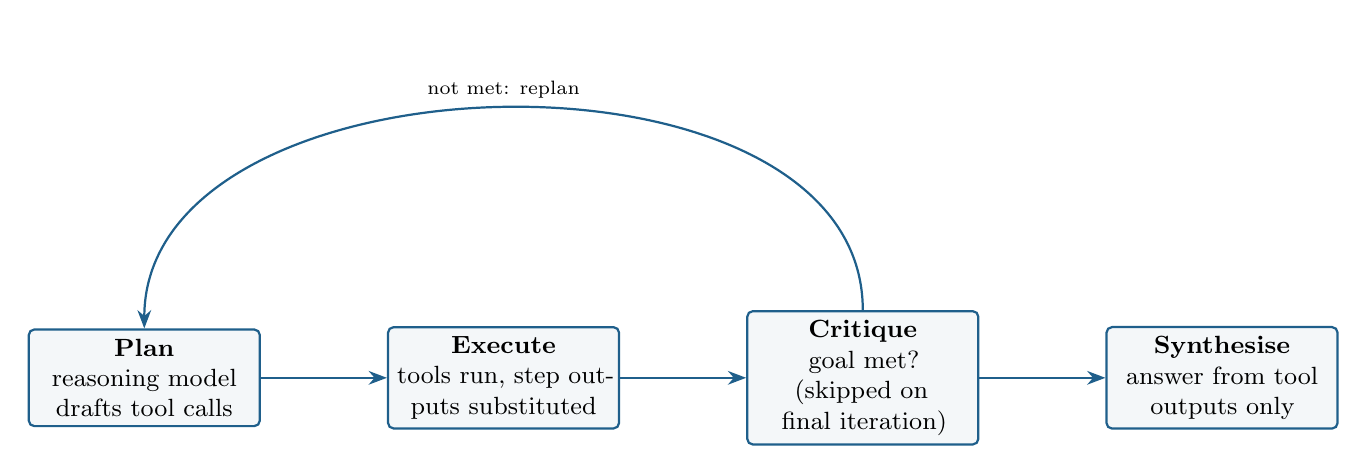
\begin{tikzpicture}[
  node distance=9mm and 16mm,
  box/.style={draw=accent, rounded corners=2pt, fill=soft, minimum height=9mm,
              text width=27mm, align=center, font=\small},
  >=Stealth, thick, accent/.style={draw=accent}]
\node[box] (plan) {\textbf{Plan}\\reasoning model drafts tool calls};
\node[box, right=of plan] (exec) {\textbf{Execute}\\tools run, step outputs substituted};
\node[box, right=of exec] (crit) {\textbf{Critique}\\goal met? (skipped on final iteration)};
\node[box, right=of crit] (synth) {\textbf{Synthesise}\\answer from tool outputs only};
\draw[->, accent] (plan) -- (exec);
\draw[->, accent] (exec) -- (crit);
\draw[->, accent] (crit) -- (synth);
\draw[->, accent] (crit.north) to[out=90,in=90] node[above,font=\scriptsize]{not met: replan} (plan.north);
\end{tikzpicture}
\end{center}

The planner never sees tool results before writing the plan, so later steps
reference earlier ones with a \code{\{\{stepN\}\}} placeholder, resolved at
execution time (\code{Agent.\_resolve}). Every tool call, its coerced
arguments, and its raw output are hash-chained into the audit log --
this is exactly what the Ask tab's Steps panel and the Audit tab display.

\subsection{Worked example, traced live}\label{sec:worked}

Query: \emph{``Which units are affected if P-101A is isolated, and draft an
approval note recommending seal replacement.''}

\begin{enumerate}
  \item Retrieval router: tag \code{P-101A} + impact word \emph{affected}
        $\Rightarrow$ \code{traverse} mode, 3-hop walk.
  \item \code{graph\_query(entity="P-101A", hops=2)} returns
        \code{E-204} (1 hop, direct \code{FEEDS}) and \code{V-1201}.
  \item \code{kb\_search} pulls the grounding text: the isolation note and the
        P-101A inspection findings (seal weepage, recommend replacement).
  \item The synthesis step composes the answer citing
        \code{[piping\_topology\_unit3 p.1]} and \code{[inspection\_report\_p101a p.1]}
        -- every claim traces to a retrieved passage, not to model memory.
\end{enumerate}

The critical property: \code{V-1201} is reachable from \code{P-101A} only by
walking \code{FEEDS} edges through \code{E-204} in the graph -- no embedding
model retrieves that connection from text similarity alone. This is the
Graph~RAG differentiator this project adds beyond the problem statement's
literal requirements.

%=============================================================================
\section{Adding New Data: The Correct Startup Procedure}\label{sec:reindex}
%=============================================================================

\subsection{Why order matters}

Ku\.zu (the graph database) permits \emph{either} many read-only handles on a
database path, \emph{or} exactly one read-write handle -- never a mix, and
never two read-write handles. The API process (\code{app/main.py}) is the only
process in this system that opens \code{data/stores/graph} in read-write mode.
\code{make index} (\code{scripts/02\_build\_index.py}) also opens it
read-write, to extract and write graph nodes/edges from new documents. \term{The
two can never run at the same time.} The Streamlit console does not open the
store at all as of 10 September 2026, so it does not need to be stopped for
this -- only the API does.

\subsection{Procedure}

\begin{enumerate}
  \item \textbf{Check ports and locks are clear} before starting or stopping
        anything:
\begin{lstlisting}[style=sh]
ss -ltn | grep -E ':8077|:8501'      # both should be free before a fresh start
fuser -v data/stores/graph            # should be empty before reindexing
\end{lstlisting}
  \item \textbf{Stop the API} if it is running (Ctrl-C in its terminal, or):
\begin{lstlisting}[style=sh]
pkill -f "uvicorn app.main:app"
\end{lstlisting}
        The Streamlit console may keep running through this step -- it will
        simply show stale numbers until you restart it, and its next call to
        the API will fail cleanly with ``cannot reach the API'' rather than a
        lock error.
  \item \textbf{Add the new documents.} Copy \code{.pdf}, \code{.txt}, or
        \code{.md} files into \code{data/corpus/} (via the Documents tab
        uploader, or directly on disk). \term{Image files} (\code{.png},
        \code{.jpg}) are \emph{not} picked up by the indexer -- they remain
        available to the vision tool on demand but are not chunked into the
        graph or vector store.
  \item \textbf{Reindex:}
\begin{lstlisting}[style=sh]
make index
# equivalent to: ./.venv/bin/python scripts/02_build_index.py
\end{lstlisting}
        This is safe to re-run: extraction is cached by chunk hash, so only
        new or changed content costs LLM time. It ingests the corpus, adds
        chunks to the vector store, extracts graph nodes/edges (LLM-driven,
        the slow step), and re-summarises communities.
  \item \textbf{Restart both services, with the port check built in:}
\begin{lstlisting}[style=sh]
make start
# equivalent to: ./scripts/06_start_all.sh
\end{lstlisting}
        This script refuses to start if port 8077 or 8501 is already
        occupied, confirms Ollama is up, starts the API, polls
        \code{/health} until it responds, and only then starts the console --
        eliminating the process-ordering problems this project hit twice
        during development.
  \item \textbf{Verify the new data landed:}
\begin{lstlisting}[style=sh]
curl -s http://127.0.0.1:8077/health
\end{lstlisting}
        Check \code{graph\_nodes}, \code{graph\_edges}, and
        \code{vector\_chunks} increased as expected, then confirm in the
        Documents tab that the new file shows \code{indexed: yes}.
\end{enumerate}

\subsection{Quick reference}

\begin{center}
\renewcommand{\arraystretch}{1.3}
\begin{tabularx}{\linewidth}{@{}l X@{}}
\toprule
\textbf{Command} & \textbf{Purpose} \\
\midrule
\code{make check} & Verify the environment (Python, models pulled, GPU) \\
\code{make index} & (Re)build vector index + knowledge graph from \code{data/corpus/} \\
\code{make start} & Port-checked, correctly-sequenced launch of API + console \\
\code{make serve} & API alone, on 8077 \\
\code{make app} & Console alone, on 8501 (requires the API already running) \\
\code{make test} & Run the 70-test suite \\
\code{fuser -v data/stores/graph} & See which process(es) hold the graph store open \\
\bottomrule
\end{tabularx}
\end{center}

%=============================================================================
\section{Grounding: What Was Fixed, and How to Verify It Yourself}\label{sec:grounding}
%=============================================================================

\subsection{The failure that was observed}

Asked to find a research paper on \emph{``Attention Is All You Need''} (which
does not exist in this corpus and cannot exist -- this machine has no internet
access), the agent: searched the knowledge base and found nothing relevant;
tried three times to fall back to a general web search, which failed every
time because the sandbox has no route out; and then, having no instruction to
do otherwise, took the closest superficially-similar document actually in the
corpus (an unrelated paper on transmission-line defect detection that happens
to mention ``attention mechanisms'') and presented \emph{that} as the answer,
complete with a real but entirely unrelated DOI link.

\subsection{Root cause}

Two gaps in \code{app/agent/loop.py}:

\begin{enumerate}
  \item The \emph{planning} prompt never told the model that internet access
        does not exist, so the planner would draft web-search steps that were
        guaranteed to fail, wasting iterations before falling through to a bad
        answer.
  \item The \emph{synthesis} prompt said only ``answer using the tool results
        below'' -- with no instruction covering the case where those results
        do not actually address the request. When the only material found was
        off-topic, the model filled the gap by presenting it as on-topic
        rather than saying so.
\end{enumerate}

\subsection{The fix}

Both prompts were made explicit:

\begin{itemize}
  \item \textbf{Planning prompt} now states: \emph{``THIS MACHINE HAS NO
        INTERNET ACCESS, EVER \dots\ if kb\_search/graph\_query cannot find
        what the request needs, the correct plan is a single step that
        reports the knowledge base has nothing relevant -- not a retry
        against the internet.''}
  \item \textbf{Synthesis prompt} now states: \emph{``If the tool results do
        not actually address the request \dots\ you MUST say plainly that it
        was not found in the knowledge base and there is no internet access
        to fetch it. Do NOT present an unrelated document as if it answers
        the request, and do NOT answer from your own training knowledge.''}
\end{itemize}

Re-running the exact same query after the fix, live:

\begin{lstlisting}[style=sh]
"answer": "The request for a research paper on \"Attention is All You
Need\" and its link was not found in the knowledge base. There is no
internet access to fetch it."
\end{lstlisting}

with zero web-search steps drafted at all.

\subsection{Important caveat -- what this fix is, and is not}

This is a \term{prompt-level instruction}, enforced by the reasoning model
following directions -- it is not a mechanical gate that makes fabrication
structurally impossible. A sufficiently different phrasing of an off-corpus
request, or a weaker/differently-tuned model, could in principle still slip
past it. The recommended hardening not yet implemented is a relevance-score
threshold on retrieval that mechanically blocks synthesis when nothing scores
above it, plus a post-hoc check that every claim in the answer traces to a
retrieved chunk. Until that lands, treat every answer as needing the
verification protocol below, not as unconditionally trustworthy.

\subsection{How to check your own project is not hallucinating}

\begin{enumerate}
  \item \textbf{Cross-check every citation.} Every grounded answer cites
        \code{[doc\_id p.N]}. Open the Documents tab, confirm that
        \code{doc\_id} is actually in \code{data/corpus/} and actually says
        what the answer claims. A citation to a document that is not listed
        there, or that does not contain the claimed fact, is a fabrication.
  \item \textbf{Run the same query in Search first.} Search is retrieval only
        -- no synthesis, so it cannot fabricate. If Search returns nothing
        relevant, the corresponding Ask answer \emph{must} be a refusal. If
        Ask instead gives a confident answer while Search found nothing, that
        is exactly the failure mode described above, recurring.
  \item \textbf{Probe with a known-absent question.} Periodically ask
        something you know is not in the corpus (a piece of general trivia,
        or a real fact about equipment that does not exist in
        \code{data/corpus/}). The correct behaviour is an explicit refusal
        citing no internet access, every time.
  \item \textbf{Read the Steps panel, not just the Answer.} Every tool call's
        raw output is shown in the Ask tab. If the final Answer states
        something the raw retrieved text does not support, that is
        fabrication even when retrieval itself found genuinely relevant
        material -- a subtler failure than citing the wrong document
        entirely.
  \item \textbf{Verify the audit chain.} The Audit tab's ``Hash chain
        verified'' status confirms the recorded trace has not been altered
        after the fact, so the Steps panel is a trustworthy record of what
        actually happened, not a reconstruction.
\end{enumerate}

\end{document}
